\textbf{Beispiel 2}\\ \\
a) \\ \\
Freigeschnittene Brücke:
\begin{figure}[h]
	\centering
	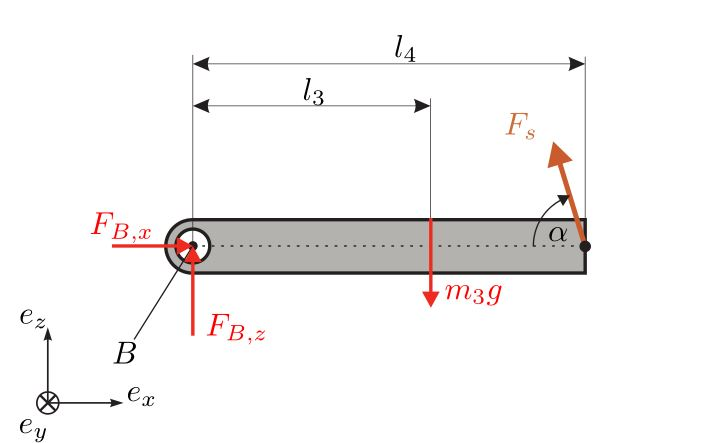
\includegraphics[width= 10cm]{tikz/08_11_2019_2a}
\end{figure}
Die Gleichgewichtsbedingungen lauten
\begin{align*}
	\textbf{e}_x &:  F_{B,x} - F_s\cos(\alpha) = 0\\
	\textbf{e}_z &: F_{B,z} - m_3g + F_s\sin(\alpha) = 0\\
	\textbf{e}_y &: -m_3gl_3 + F_s\sin(\alpha)l_4 = 0
\end{align*}
\newpage
\noindent
Aus diesen Gleichungen erhaltet man für die Kräfte
\begin{align*}
	F_s &= \frac{m_3gl_3}{\sin(\alpha)} \\
	F_{B,x} &= F_s\cos(\alpha) = \frac{m_3gl_3}{\tan(\alpha)} \\
	F_{B,z} &= m_3g - F_s\sin(\alpha) = m_3g\left(1 - \frac{l_3}{l_4}\right)
\end{align*}
b)\\ \\
Die beiden Massen lauten
\begin{align*}
	m_1 &= \rho_1 l_1A \\
	m_2 &= \rho_2 l_2A
\end{align*}
Die Lagen der beiden Schwerpunkte lauten
\begin{align*}
	l_{1,s} &= -\left(\frac{l_1}{2} + l_c\right) \\
	l_{2,s} &= \frac{l_2}{2} - l_c
\end{align*}
c) \\ \\
Die gesamte Masse lautet
\[
	m_g = A(l_1\rho_1 + l_2\rho_2)
\]
Die Position des resultierenden Schwerpunkt wird mit der Formel \textit{Schwerpunkt eines zusammengesetzten Körpers} aus der Formelsammlung ermittelt. Diese lautet daher
\[
	l_g = \frac{-l_1(l_1 + 2l_c)\rho_1 + l_2(l_2 - 2l_c)\rho_2}{2(\rho_1l_1 + \rho_2l_2)}
\]
d)\\ \\
Freigeschnittener Träger:
\begin{figure}[h]
	\centering
	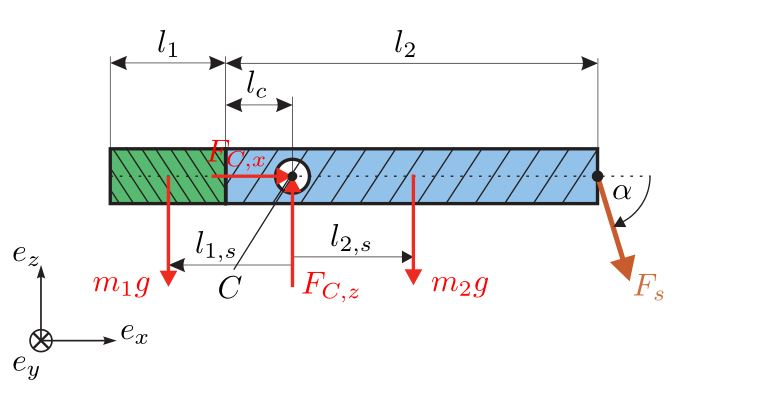
\includegraphics[width=10cm]{tikz/08_11_2019_2d}
\end{figure}
\newpage
\noindent
Die Gleichgewichtsbedingungen hier lauten
\begin{align*}
	\textbf{e}_x &: F_{C,x} + F_s\cos(\alpha) = 0\\
	\textbf{e}_z &: F_{C,z} - m_1g - m_2g - F_s\sin(\alpha) = 0\\ 
	\textbf{e}_y &: m_1gl_{1,s} - m_2gl_{2,s} - F_s\sin(\alpha)l_s = 0
\end{align*}
Aus den ersten beiden Gleichungen folgen für die Kräfte in Lager C
\begin{align*}
	F_{C,x} &= -\frac{m_3gl_3}{\tan(\alpha)} \\
	F_{C,z} &= g\left(A(l_1\rho_1 + l_2\rho_2) + \frac{l_3m_3}{l_4}\right)
\end{align*}
e) \\ \\
Aus der Momentenbilanz für den Träger folgt durch Umformen
\[
	l_1 = -l_c + \sqrt{l_c^2 - \frac{2m_2l_{2,s}}{\rho_1A} - \frac{2F_s\sin(\alpha)(l_2 - l_c)}{\rho_1Ag}}
\]